\documentclass[xcolor=dvipsnames]{beamer}
\usecolortheme[named=NavyBlue]{structure}
\usetheme{Berlin}
\usepackage{graphicx}
\title{Understand Machine Learing}
\author{}
\institute{}
%\date{2021-12-24}
%%%%%%%%%%%%%%%%%%%%%%%%%%%%%%%%%%%%%%%%%%%%%%%%

\usepackage{amsmath, amsthm, amsfonts, amssymb}
\everymath{\displaystyle}
%%%%%%%%%%%%%%%%%%%%%%%%%%%%%% Textclass specific LaTeX commands.
\theoremstyle{plain}
\newtheorem{thm}{\protect\theoremname}[section]
\newtheorem{cor}[thm]{Corollary}
\newtheorem{lmma}[thm]{Lemma}
\newtheorem*{defn}{\underline{Definition}}
\newtheorem*{ex*}{Example}
\newtheorem*{sol*}{Solution}
\newtheorem*{thm*}{Theorem}
\newtheorem*{lmma*}{Lemma}
\newtheorem*{rmk*}{Remark}
\newtheorem*{pf*}{\underline{\textbf{Proof\ }}}

%%%%%%%%%%%%%%%%%%%%%%%%%%%%%% User specified LaTeX commands.
\renewcommand{\P}{\mathscr{P}}
\newcommand{\B}{\mathscr{B}}
\newcommand{\A}{\mathscr{A}}
\newcommand{\C}{\mathbb{C}}
\newcommand{\CC}{\mathscr{C}}
\newcommand{\R}{\mathbb{R}}
\newcommand{\Q}{\mathbb{Q}}
\newcommand{\Z}{\mathbb{Z}}
\newcommand{\N}{\mathbb{N}}
\newcommand{\X}{\mathcal{X}}
\newcommand{\T}{\mathscr{T}}
\newcommand{\arbuni}{\bigcup_{\alpha\in I}}
\newcommand{\finint}{\bigcap_{i=1}^n}
\newcommand{\Ua}{{\textsc{U}_\alpha}}
\newcommand{\Ui}{\textsc{U}_i}
\newcommand{\pair}[2]{\left( \,#1\,,\,#2\,\right) }
\newcommand{\sett}[1]{\left\{#1 \right\}}
\newcommand{\dint}[2]{\int_{#1}^{#2}}
\DeclareMathOperator*{\esssup}{ess\,sup}

%%%%%%%%%%%%%%%%%%%%%%%%%%%%%%
\begin{document}

	\begin{frame}
    	\titlepage 
	\end{frame}

\begin{frame}
	\tableofcontents	
\end{frame}

% Presentation structure

\begin{frame}
	\section{Road Map}
	Road Map
	
	\begin{center}
		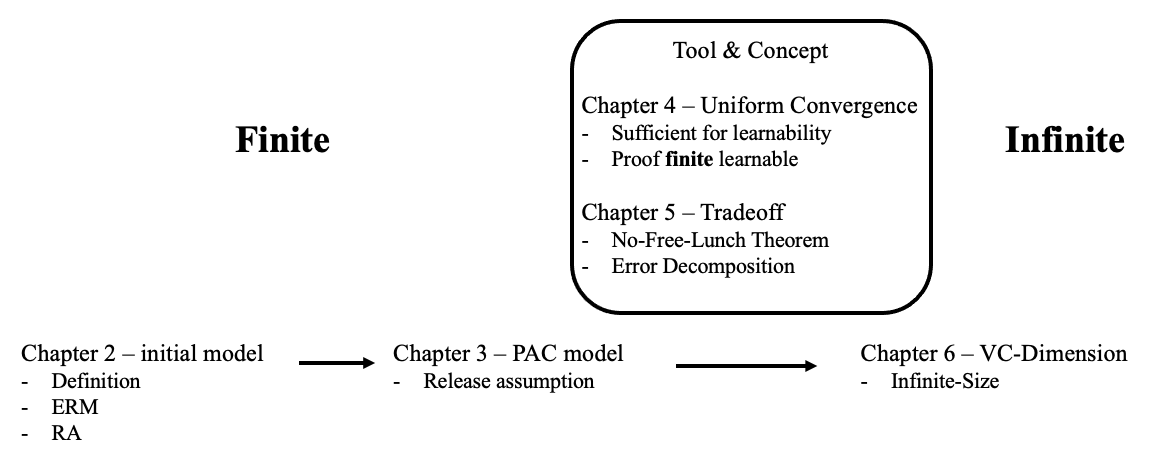
\includegraphics[scale = 0.25]{./figure/0-1.png}
	\end{center}
    
\end{frame}

\begin{frame}
	\section{A Gentle Start}
	\frametitle{Definition}
	\textbf{Domain set:} An arbitrary set, $\chi$. This is the set of objects that we may wish to label.
\end{frame}

\begin{frame}
	\frametitle{Definition}
	\textbf{Label set:} The Answer of the Domain set, usually $\sett{0,1}$ or $\sett{-1,+1}$
\end{frame}

\begin{frame}
	\frametitle{Definition}
	\textbf{Training data:} $S = ((x_1,y_1),\cdots,(x_m,y_m))$ is a sequence of labeled domain points.
\end{frame}

\begin{frame}
	\frametitle{Definition}
	$h:\chi \rightarrow y,$ a prediction function, also called a predictor, hypothesis, classifier.
\end{frame}


\begin{frame}
	\frametitle{Definition}
	Formally, the learner should choose tin advance a set of predictors. This set is called a hypothesis class and is denoted by $H$. Each $h \in H$ is a function mapping from $\chi$ to $y$.
\end{frame}


\begin{frame}
	\frametitle{Definition}
	\textbf{A data-generation model:} We now explain how the training data is generated by som probability distribution. Let us denote that probability distribution over $\chi$ by $D$.
	
\end{frame}

\begin{frame}
	\frametitle{Definition}
	\textbf{Measure of Success:} To know is the output is good or not, we define the loss function to check it
	
\end{frame}

\begin{frame}
	\frametitle{Definition}
	\begin{enumerate}
		\item \textbf{True error:} $L_{D,f}(h) = \mathbb{P}_{x\sim D}[h(x) \neq f(x)] = D(\sett{x ~|~ h(x) \neq f(x)})$
		\item \textbf{Training error:} \\ $L_S(h) = \dfrac{|\sett{i \in m ~|~ h(x_i) \neq y_i} |}{m}$ where $[m] = \sett{1,\cdots,m}$
	\end{enumerate}
	
\end{frame}

\begin{frame}
	\frametitle{Definition}
	\begin{center}
		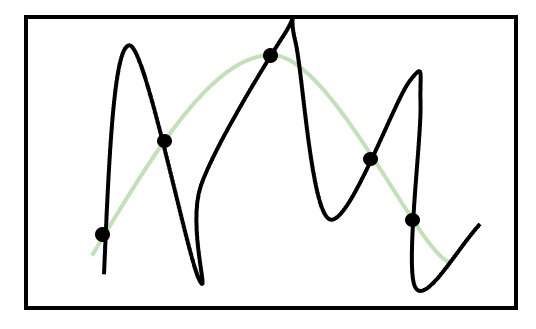
\includegraphics[scale = 0.3]{./figure/2-1.png}
		
		Figure 2-1, training error is $0$ but true error is bad
	\end{center}
	
\end{frame}


\begin{frame}
	\frametitle{Definition}
	\begin{enumerate}
		\item[$\cdot$] We denote the probability of getting a non-representative sample by $\delta$, and call ($1 - \delta$) the \textbf{confidence parameter} of our prediction
		\item[$\cdot$] The \textbf{accuracy parameter}, commonly denoted by $\epsilon$. We interpret the event $L_{(D,f)}(h_s) > \epsilon$ as a failure of the learner
	\end{enumerate}
	
\end{frame}

\begin{frame}
	\section{Improve Model}
	\frametitle{Empirical Risk Minimization}
	
	The method to proof the model is to minimize the loss function by using training data, i.e. we check $L_S(h)$
	
\end{frame}

\begin{frame}
	\frametitle{Empirical Risk Minimization}
	The $\text{ERM}_H$ learner uses the ERM rule to choose a predictor $h \in H$, with the lowest possible error over $S$. Formally

$$h_S = \text{ERM}_H(S) \in \arg\min_{h \in H}L_S(h)$$
	
\end{frame}

\begin{frame}
	\frametitle{Overfitting}
	cause by ERM, the data is too fit the training set

example: $h_s(x) = \begin{cases}
	y_i~\text{if}~\exists~i \in [m]~\text{s.t. } x_i = x\\
	0~\text{otherwise}
\end{cases}$
	
\end{frame}


\begin{frame}
	\section{The upper bound of $L_{(D,f)}(h_s)$ in finite hypothsis}
	\frametitle{Inductive bias}
	Restricting the learner to choosing a predictor from $H$ are often called an \textbf{inductive bias}. In following statement, we will proof that when we have some assumption, $H$ is a finite set and have enough quantity of data set, then we can avoid the overfitting problem.
	
	
\end{frame}


\begin{frame}
	\frametitle{Some assumption}
	\textbf{The Realizability Assumption:} There exists $h^* \in H$ s.t. $L_{(D,f)}(h^*) = 0$. Note that this assumption implies that with probability $1$ over random samples, $S$ where the instances of $S$ are sampled according to $D$ and are labeled by $f$, we have $L_S(h^*) = 0$

	
\end{frame}


\begin{frame}
	\frametitle{Some assumption}
	\textbf{The i.i.d. assumption :} The examples in the training set are independently an identically distributed (i.i.d) according to the distribution $D$. We denote this assumption by $S \sim D^m$ where $m$ is the size of $S$, and $D^m$ denotes the probability over $m$-tuples induced by applying $D$ to pick each element of the tuple independently of the other members of the tuple.
	
\end{frame}


\begin{frame}
	\frametitle{Proof Section}
	The goal is to proof when $m \geq \dfrac{\log(|H|/\delta)}{\epsilon}$, then $L_{D,f}(h_s) \leq \epsilon$
	
\end{frame}

\begin{frame}
	\frametitle{Proof Section}
	Let $H_B$ be the set of "bad" hypotheses, that is,

$$H_B = \sett{h \in H~|~L_{D,f}(h)>\epsilon}$$
	
\end{frame}


\begin{frame}
	\frametitle{Proof Section}
	In addition, let

$$M = \sett{S|_x ~|~ \exists~h \in H_B,L_S(h) = 0}$$

be the set of \textbf{misleading sample}(they are bad but $L_S(h_S) = 0$)
	
\end{frame}


\begin{frame}
	\frametitle{Proof Section}
	by definition, we can write 

$$\sett{S|_x ~|~ L_{(D,f)}(h_S) > \epsilon} \subseteq M\color{red}(\star_1) $$


We can rewrite $M$ as (thought it's intersection was not empty)

$$M = \cup_{h \in H_B}\sett{S|_x ~|~ L_S(h) = 0}\color{red}(\star_2)$$
	
\end{frame}


\begin{frame}
	\frametitle{Proof Section}
	by $(\star_1),(\star_2)$,

$$D^m(\sett{S|_x~|~L_{(D,f)}(h_s)>\epsilon}) \leq D^m(M) $$

$$= D^m(\cup_{h\in H_B}\sett{S|_x ~|~ L_S(h) = 0})\color{red}(\star_3)$$
	
\end{frame}


\begin{frame}
	\frametitle{Proof Section}
	\textbf{LEMMA}(Union Bound) For any two sets $A,B$ and a distribution $D$ we have

$$D(A\cup B) \leq D(A) + D(B)$$
	
\end{frame}


\begin{frame}
	\frametitle{Proof Section}
	and the $(\star_3)$ can be bound like this

$$D^m(\sett{S|_x ~|~ L_{(D,f)}(h_S)>\epsilon}) \leq \sum_{h \in H_B}D^m(\sett{S|_x ~|~ L_S(h) = 0})\color{red}(\star_4)$$
	
\end{frame}


\begin{frame}
	\frametitle{Proof Section}
	\textbf{Next, we fix $h_B$ on the bad hypothesis $h_B \in H_B$} $\implies L_{(D,f)}(h) > \epsilon$
	
\end{frame}


\begin{frame}
	\frametitle{Proof Section}
	because the event are i.i.d, we get that

$D^m(\sett{S|_x~|~L_S(h)=0}) = D^m(\sett{S|_x ~|~\forall i,h(x_i) = f(x_i)})$

$ = \prod^m_{i=1}D(\sett{x_i~|~h(x_i) = f(x_i)})\color{red}(\star_5)$
	
\end{frame}


\begin{frame}
	\frametitle{Proof Section}
	check the each individual sampling of an element of the training set, we have

$D(\sett{x_i~|~h_B(x_i) = y_i}) = 1-D(\sett{x ~|~ h_B(x) \neq f(x)})$

$=1 - L_{D,f}(h_B) \leq 1 - \epsilon$
	
\end{frame}

\begin{frame}
	\frametitle{Proof Section}
	put it to the $\color{red}(\star_5)$ and use the inequality $1 - \epsilon \leq e^{-\epsilon}$

$$D^m(\sett{S|_x~|~ L_S(h_B) = 0}) \leq (1 -\epsilon)^m \leq e^{-\epsilon m}\color{red}(\star_6)$$
	
\end{frame}

\begin{frame}
	\frametitle{Proof Section}
	$D^m(\sett{S|_x ~|~L_{(D,f)}(h_s)>\epsilon}) = |H_B|D^m(\sett{{S|_x ~|~L_S(h_B)=0}})$
	
	$|H_B|$ means the cardinality(element number) of $H_B$
	
\end{frame}


\begin{frame}
	\frametitle{Proof Section}
	put $\color{red}(\star_6)$ back to $\color{red}(\star_4)$ 
	
	$$D^m(\sett{S|_x ~|~ L_{(D,f)}(h_S)>\epsilon}) \leq |H_B|e^{-\epsilon m} \leq |H|e^{-\epsilon m}$$
	
\end{frame}


\begin{frame}
	\frametitle{Proof Section}
	In this equation, we can know that when $m$ increase, the  overfitting hypothesis's probability (where the hypothesis of $L_S$ is small but $L_{(D,f)}$ is big, i.e. $D^m(\sett{S|_x ~|~ L_{(D,f)}(h_S)>\epsilon})$) will decrease.
	
\end{frame}

\begin{frame}
	Since $D^m(\sett{S|_x ~|~ L_{(D,f)}(h_S)>\epsilon})$ is $\delta$, and have a nature log, we get

$$m \geq \dfrac{\log(|H|/\delta)}{\epsilon}$$
\end{frame}

 
\end{document}
